\documentclass[11pt,a4paper]{article}
\usepackage[utf8]{inputenc}
\usepackage[T1]{fontenc}
\usepackage[french]{babel}
\usepackage[margin=1.5cm]{geometry}
\usepackage{graphicx}
\usepackage{hyperref}
\usepackage{enumitem}
\usepackage{titlesec}

\setlist{nosep,leftmargin=1.2em}
\titlespacing*{\section}{0pt}{0.4em}{0.2em}
\titleformat{\section}{\normalfont\bfseries\large}{\thesection}{0.5em}{}
\setlength{\parskip}{0.2em}
\setlength{\parindent}{0pt}

\title{\vspace{-1.5cm}Rapport individuel --- It\'eration 2}
\author{Mati Afriat (\texttt{mat6784}) --- Projet Long SHDL}
\date{11 mai 2026}

\begin{document}
\maketitle
\vspace{-2em}

\section*{Contexte}
Responsable du \textbf{simulateur} (axe \emph{simulation}, branche \texttt{simulation}). Objectif sprint~2~: faire converger les deux mod\'elisations explor\'ees au sprint~1 vers une \emph{interface unique} consommable par le parser d'Alexis, et \'etendre le langage support\'e (op\'erations logiques, vecteurs de signaux, appel de module). Construction d'une nouvelle abstraction \texttt{Erwan} servant de pivot entre interpr\'etation et simulation.

\section*{Activit\'es r\'ealis\'ees}
\begin{itemize}
  \item \textbf{Package \texttt{erwan/}} (interface interpr\'etation/simulation)~: classe \texttt{Erwan} mod\'elisant un signal comme une op\'eration arborescente (un \texttt{Erwan} contient les autres \texttt{Erwan} dont il d\'epend + l'\texttt{Operation}), interface \texttt{Branchement}, \texttt{AppelModule} pour la composition, \texttt{Operation \{ET, OU, NON, XOR, IDENTITE, CONSTANTE\}}, \texttt{Descripteur} pour les vecteurs (range \texttt{indiceDebut}..\texttt{indiceFin}).
  \item \textbf{Conteneur \texttt{Module}}~: agr\`ege \texttt{Plan: List<Erwan>}, \texttt{Entrees}/\texttt{Sorties: List<Descripteur>}, \texttt{Branchements: List<AppelModule>}. Contrat consomm\'e par \texttt{Conversion.convert} c\^ot\'e parser.
  \item \textbf{Support des vecteurs} (commit \texttt{vecteur fonctionnels}, 8 mai) et renforcement du simulateur historique~: \texttt{Constante}, \texttt{ConnecteurListener}, classes \texttt{Experience1..6} pour validation exp\'erimentale.
  \item \textbf{Documentation JavaDoc} g\'en\'er\'ee (\texttt{erwan/*.html}, \texttt{simulateur/*.html}).
\end{itemize}

\section*{R\'esultats}
\begin{itemize}
  \item \textbf{Interface \texttt{erwan.Module} stabilis\'ee}~: utilis\'ee comme cible par la conversion d'Alexis, tests bout-en-bout verts sur \texttt{ET}/\texttt{OU}/\texttt{NOT}/\texttt{XOR}.
  \item \textbf{Vecteurs fonctionnels} (commit \texttt{3993b11})~: ouvre la voie au support des bus dans la suite du projet.
  \item Un \textbf{bug \texttt{Erwan.OR()} retournant \texttt{Op.AND}} a \'et\'e d\'etect\'e c\^ot\'e parser via un test e2e \texttt{XOR}~; correction int\'egr\'ee au sprint avec test sentinelle.
\end{itemize}

\begin{center}
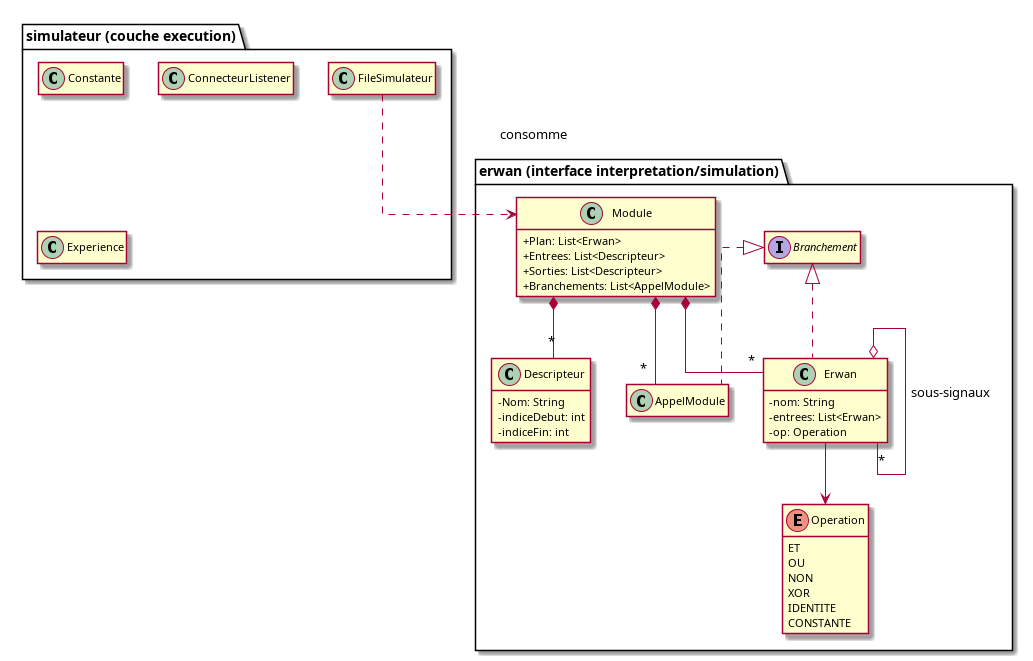
\includegraphics[width=0.42\textwidth]{mati-sprint2-classes.png}\\
{\small Figure --- Diagramme de classes du package \texttt{erwan} (source \texttt{mati-sprint2-classes.puml}).}
\end{center}

\section*{Difficult\'es et r\'eussites}
Difficult\'e~: \textbf{r\'econcilier les deux mod\`eles} du sprint~1 (Lien simple mais sans vecteurs/composition~; Connecteur expressif mais lourd). La classe \texttt{Erwan} a \'et\'e construite comme \emph{descripteur d\'eclaratif} (qui d\'epend de quoi, via quelle op\'eration) ind\'ependant de l'ex\'ecution. R\'eussite~: ce pivot rend l'int\'egration avec le parser triviale et a permis la livraison de \emph{parse~$\to$ convert~$\to$ simulate} bout-en-bout.

\section*{Manuel utilisateur}
Pr\'e-requis~: JDK~25, JUnit~4 et Hamcrest. Cr\'eation d'un \texttt{Module}~: instancier les \texttt{Erwan} via les m\'ethodes de classe (pas de constructeur public), pr\'eciser \texttt{Entrees}/\texttt{Sorties} via \texttt{Descripteur}, passer le tout \`a \texttt{new FileSimulateur(module.Plan)}. Tests~: \texttt{java org.junit.runner.JUnitCore erwan.TestErwan}. JavaDoc consultable dans \texttt{erwan/*.html} et \texttt{simulateur/*.html}. Code sur la branche \texttt{simulation}.

\end{document}
